\chapter{Related Work}
% \section{Related Work}

It is only through the recent development of large open source datasets and the techniques to process them, that statistical approaches to code-related tasks have been available to machine learning researchers. 
As would be expected of any new and growing field, the range of attempted tasks is still expanding. 


As of writing no formal attempt has been made to automatically generate natural language descriptions of individual elements of code from its source.  
This is not surprising given how recently the field has developed, and the lack of a suitable dataset.
However, progress has been made in the related fields of source code summarization, variable naming, documentation generation, and code language modelling \citep{allamanis_survey_2017}.  
These advances highlight possible approaches to statistically modelling structure of code like language.  

In this review we summarise the current advances of these methods and how they relate to the task at hand.  We start by examining progress in the language modelling of code, then examine sequence generation tasks, such code comment prediction, code summarization or function naming. We then examine advances in the fields of representation of programs and abstract syntax trees. Finally we present an overview the existing datasets and the scope of the problems they are suitable to address, finding them lacking in our particular domain.


% As mentioned in the Introduction, it is only through the recent development of large open source datasets that statistical approaches to code related tasks have been available to machine learning researchers. 
% As would be expected of any new and growing field, the range of attempted tasks is still expanding. 
% Although as of writing no formal attempt has been made to translate fine grained elements of source code into their natural language descriptions, a great deal of relevant insight has been made in the related fields of source code summarization, variable naming, documentation generation, and code language modelling. Many of these problems highlight possible approaches to modelling the patterns and structure of code as language, and can even be cast into a machine translation framework.  

% In this review we summarise the current advances of these methods and how they relate to the task at hand.  We start by examining with the general progress in the language modelling of code, before moving on to specific tasks that can be posed as sequence generation tasks, such code comment prediction, code summarization or function naming. We subsequently examine advance in the related fields of representation of programs, before we finally examine the existing datasets, and the scope of the problems they are suitable to address. 

\section{Language Models of Source Code}

The earliest work modelling source code with natural language techniques comes from Hindle at al \cite{Hindle:2012:NS:2337223.2337322}, who used simple Kneser-Ney smoothed n-gram models of code tokens, to create language models for large-scale Java and C projects.
With these models, Hindle was able to demonstrate that the cross-entropy of source code within projects was lower than that of large English corpora - indicating the presence of repetetive common patterns that could be leveraged for code completion, naming and summarization.
This was consistent with findings by Gabel and Su \cite{gabel_study_2010} who examined the lines of approximately 6000 projects of code and found widespread repetition of sections of up to several lines, both within and across projects.
Despite the simplistic Markov chain assumption implicit in the ngram model, the effectiveness of this modelling techniques, especially within projects, opened up the field of code analysis to the wider natural language processing community.

Hindle's model, which only took into the lexical structure of code, was improved by Nguyen et al\cite{nguyen_statistical_2013}, by integrating semantic information into the n-gram model.
Instead of training on the raw string of the token, the \textit{lexeme}, this model condensed information such as data type, scope, role (such as literal, variable, function call) into a \textit{sememe}, and trained an n-gram topic model, modelling both local context \textit{sememes} ngrams, and global trends in the code.
This highlighted the value of taking into account the semantic information in code, as well as the lexical, in prediction tasks.

Since then a number of different language models of code have been developed, largely finding their use in code-completion tasks. These have demonstrated the importance of factoring in the long range dependencies of code, and elements of the code beyond simple lexical structure. For instance Tu et al added a cache mechanism to improve Hindle's ngram model in capturing longer range dependencies  \cite{tu_localness_nodate}, while this itself was surpassed (up to 9 grams) with a recurrent neural language model by White et al\cite{white_toward_2015}.
Most recently, Bhoopchand et al used a sparse pointer network to create a language model that significantly outperformed a LSTM baseline on code completion tasks, that was able to refer to objects in code over 60 tokens previous\cite{bhoopchand_learning_2016}.

This work in language modelling has direct applicability to our task at hand, as it points out relevant strategies in picking out the statistically important features of `natural' code. In particular we note the importance of capturing long range dependencies (as seen in neural models), with the performance benefit that can be brought by taking into account semantic information (from the instructions given to the computer).

\section{Sequence Generation from Source Code}

A long running task is that of code summarization. 
This task involves taking large sections of code blocks, and summarising its meaning in natural language. It has historically had parallels with the long running (inverse) problem of semantic parsing. CITE
As such, early approaches to this problem completely ignored the `naturalness' properties of code and its comments, and instead was tackled with rule-based methods. 

Work by Sridhara et al \cite{sridhara_[not_2010}  used static analysis to find important semantic subunits of code in Java projects, and used sets of sentence templates to produce English from these subunits.
% This model revolved around automatic rule-based summarization of the source code in the source code in consideration.
This work produced text that describe the functions in question to a high degree of accuracy, but Sridhara noted the potential lack of transferrability to other settings, and lack of examples with which to compare their summaries.  
This procedure was also inherently inflexible, relying on human crafted templates, and specified rules. Furthermore the size of the dataset, four projects in total, indicated a potential problem in the generalisability of the work to other domains, projects or even languages.

However, the advent of the statistical approaches to code language modelling led by Hindle et al \cite{Hindle:2012:NS:2337223.2337322} signalled the start of similar approaches to sequence generation. The earliest is Movshovitz-Attias et al \cite{movshovitz-attias_natural_nodate}, who used both ngrams and topic models such as LDA to predict comments from JAVA source code. In this they found that modelling the lexical components of source code as coming from a mixture of topics - "code" and "text" - outperformed models that ignored this distinction.  This pointed to the strength of taking into account features of code (such as distinguishing comments from commands), even if such destinction were still purely on the lexical level.

% Since then, statistical approaches have become more popular in attacking the problem, often involving much larger corpora of training data.
% Iyer et al \cite{iyer_summarizing_2016} sourced a large dataset of code snippets and questions from Stack Overflow, a popular programming website, to attempt this problem statistically.
Since then neural models have become popular methods of attacking sequence generation, as they capture long range dependencies in sequences, and have shown great promise in other neural translation tasks.

A particularly successful example is that of Iyer et al \cite{iyer_summarizing_2016}, who applied a neural attentional model to the problem of generating code `summaries'. This model trainied on a large collection of snippets and questions from Stack Overflow, a programming help website.   Iyer's model combined two features: a distributed representation of the code, generated by an attentional mechanism \cite{luong_effective_2015} over code token embeddings; and an LSTM unit \cite{hochreiter_long_1997} to encode natural language tokens. Together these generated descriptions as a sequence of conditional distributions, in an encoder-decoder model. 

As usual, this model calculated the probability of generating a length $l$
descriptive sequence $\{y_1,...,y_l\}$ through a product of conditional probabilities of the previous $l-1$ tokens:

$$P(y_1,...,y_l| \mathcal{C}) = \prod_{i=1}^lp(y_i | y_1, ..., y_{i-1}, \mathcal{C} ) $$

In this case, each conditional probability was proportional to a non-linear transformation of the combination of hidden state of the LSTM $\mathbf{h_i}$ and the attentional vector  $\mathbf{t_i}$ at that point in the sequence: 

$$\text p(y_i | y_1, ..., y_{i-1},\mathcal{C} ) = g(\mathbf{h_i}, \mathbf{t_i}) $$
$$g(\mathbf{h_i}, \mathbf{t_i})  \propto \mathbf{W}\text{tanh}(\mathbf{W_1h_i} + \mathbf{W_2t_i})$$

where $\mathbf{W} \in \mathbb{R}^{|N|\text{x} H}, \mathbf{W_1}$ and $\mathbf{W_2} \in \mathbb{R}^{H \text{x} H}$  and $ H$ is embedding dimensionality of words, $ N $ the vocabulary.\cite{iyer_summarizing_2016}
A visual schematic of the model is preseted in Figure \ref{fig:Iyer}.

Iyer et al then ran a beam search over the decoder to explore the space of likely sequences, and evaluated their generations using the BLEU-4 and METEOR metrics.

Iyer's model achieved a new record in the performance of the code summarization task. 
It outperformed rival NLP models such as MOSES, a phrase-based translation model \textbf{CITE \& paraphrase}, and SUM-NN, another attention based summarization model using dense layers instead of LSTMs. 
It also achieved a first in learning to generate original sentences from arbitrary code sections, and has proved successful in other domains.  

Loyola et al \cite{loyola_neural_2017}, for instance, adapted a similar attention model to Iyers to generate short descriptions of differnces in code.
This time intead of training on a single piece of source code and questions, data was sourced to present pairs of code changes (`diffs') with comments describing the change (`commit messages'). 
In this setting, the attentional model was able to generate faesible messages, both within projects and between projects.

These attention models show the effectiveness of being able to pickout relevant portions of code at different points in sequence generation, but fail to take into account the longer term correlations of the tokens in source code. In fact by only processing source code with this kind of attention, both models treat the source code as little more than bag of token embeddings.

In this regard, an improvement on these attentional models is that of Alamanis et al \cite{allamanis_convolutional_2016}, which uses a convolutional attention network over tokens, for the task of predicting the names of functions given their body. This is cast as `extreme summarization'.
%aiming to capture long range correlations in code through spatial convolutions instead of temporal hidden state.

In this model source code is split lexically into a padded sequence of embedded tokens, over which a one-dimensional convolution of fixed-width is run, creating a number of attentional feature vectors $\mathbf{\{v_k\}}$.
These feature vectors are then element-wise multiplicatied with the hidden state of an rnn, $\mathbf{h_{t-1}}$, to be effectively `selected' for their relevance to next generated token. They are then normalised.

This set of feature vectors is then convolved with an attention kernel, to give a set of attention weights, each corresponding to a token embedding. 
A final attention vector $\mathbf{\alpha}$ is constructed from the convex combination of the token embeddings under the attention weights, and this vector is used to generate a distribution over the next function subtoken.
An illustration of the algorithm with pseudo code is presented in Figure X.

The authors of this model apply it to both the narrow task of generating function names, and that of code retrieval. In it they find that taking into account the long range features of the code in the convolutional model surpasses a baseline attentional model of the machine translation model originated by Bahdenau \cite{bahdanau_neural_2014}, and found that this performance was further improved by adding a cacheing mechanism to the model.

Both these attention models show the strengths that attention can provide in combining the modalities of text and code. However, a key failing of both models remains their lack of appreciation for the syntax and semantics of the underlying code.
Although Allamanis et al's model is more aware of the structure of lexical code tokens than Iyer et als, both models continue to ignore a fundamental channel of information communication through code - that of communication from human to computer.

% Other forms of machine translation? 
% Phrase based translation, 
% neural mthods, 
% pseudo code

As of writing no published work has been applied to generating documentation of source code using the syntactical structure of source code.  However, a number of pieces of work have recently started to examine such structure in other tasks. These are the topics of the next section of review.

\section{Syntactic Representations of Source Code}

A number of probablistic models have attempted to capture the the syntax of code, outside of the field of documentation generation.
Raychev et al \cite{raychev_probabilistic_nodate} use decision trees to develop the probabilistic model of code from the syntax tree, in a code-completion setting. 
Maddison and Tarlow \cite{maddison_structured_2014} use probabilistic context free grammars to model the AST, for a generative model. 
Neither of these approaches provides us with the natural structure we can easily use for sequence generation. 

Allamanis et al models the AST as explicitly as a graph, adding extra edges such as "guarded by", or "last lexical use", to capture additional semantic information\cite{allamanis_learning_2017}. These graphs are then processed with a Gated Graph Neural Network in a variable naming and variable misuse classification task. 
This last method proves remarkably effective, though it appears highly complex to implement, the additional semantic annotations added can appear particularly arbitrary. As a result of both of these, we avoid using these representations as inputs for our task.

A simpler way to capture the syntax of the code is to reparameterise the AST.
Since a tree can be fully specified by the set of shortest paths between all leaf nodes, an AST can now be treated as bag of these paths. This was the parameterisation was proposed by Alon et al in 2018 \cite{alon_general_2018}, and has since been applied successfully in a function name classification context\cite{alon_code2vec_2018}.

In this model, codepaths are parameterised into `path-contexts' - triples of the two terminal node names and the specific paths connecting them.
Each path and terminal node has a respective embedding (learnt alongside the main task), and for each path-context, the repective two terminals and path are concatenated and fed through a neural-network layer to combine into a single path-context vector.
A general code vector is then produced from a simple attention mechanism over the every path-context vector in the tree. 


Alon et al are able to demonstrate a performance in a function name classification task that surpasses both Allamanis et als' \cite{allamanis_convolutional_2016} and Iyer et als \cite{iyer_summarizing_2016}. This simplicity and proven effectiveness demonstrate an appealing approach to capturing semantics within the structure of with AST.

\section{Existing Datasets}
\label{sec:existing_datasets}

The scope of the tasks available to challenge researchers is naturally limited by the set of available datasets.
% Given the relative novelty of the field, there still a limitation in the number of datasets that have been collected, cleaned and are suitable for certain tasks.
In this section we outline the current state of the available datasets for researchers looking to generate sequences from source code. In doing so we indicate why none so far is suitable our task of generating documentation or summaries from fine-grained elements of source code.

\subsection{Stack Overflow Dataset}

A commonly used dataset for code captioning and summarization tasks is sourced from a large corpus of questions and code snippets from the programming help website Stack Overflow, as generated by Iyer et al\cite{iyer_summarizing_2016}. In it, questions such as ``how do I concatenate entire result sets in mysql? ' are paired with the snippets of C\# or SQL which are responses to the question, posted by other users online.
Although widely used, this dataset suffers from a number for undesirable features for our task. 

First of all the preparation of such a dataset demonstrates a lot of arbitrary cleaning.
Since many of the responses from the website are invalid or do not quote code, the snippets in question have been found by searching for html \mintinline[]{python}{<code>} tags in the upvoted answers. 
The authors note that these sections of code often bore no real relevance to the question at hand. Therefore the authors were forced to train a semi-supervised classifier to filter only relevant snippets to the question at hand.
This convoluted pipeline runs the risk of increasing the number anomalous datapoints in the dataset, whilst reducing almost a million (query,snippet) pairs from each language, down to 66,000 pairs  of C\# and 32,000 pairs of SQL.

Furthermore, the authors noted that often the informal code snippets often contained syntactic errors, with only 12\% of SQL snippets parsing without syntactic error. They progress with a best-effort parse, but this
 lack of code quality, naturally poses a problem for our fine grained analysis of code segments, or indeed any analysis using the syntactical properties of code.

Finally the dataset itself lacks a lot of the context and information needed for the granular analysis necessary for individual sections of code. Not only is the natural language not tailored to specific parts of the code, but the artificial snippets lack a lot of the context of real `natural' codebases. In fact, given the snippets' only relevant context is that of the question, the authors are forced to mask items like string literals and the like, to prevent the close context of the question and nothing else. This modification of the code is also undesirable.

Naturally in our search for an appropriate code base, we seek larger bigger elements of `real' (and fully parsing) code, with appropriate descriptions of elements, and a greater sense of `naturalness'.

\subsection{Edinburgh Corpus}

A recent corpus specifically tailored to code-to-text generation, is one of Python code as released by Barone and Senrich \cite{barone_parallel_2017}, which we refer to as the Edinburgh Corpus. 
This is a set of 109,000 triplets of function declarations, bodies, and documentation strings (docstrings), scraped from the most popular projects in GitHub, using the same methodology as Bhoopchand et al. 

In this dataset, the authors focus on finding real world code, and extracting the string, written by code authors, providing a description of each function.
Although these source code sections and natural language strings are more `natural' than their Stack Overflow counterparts, they still don't suit our needs, mainly in the form of the language they provide. 

The Python language enforces no constraints on the content or format of the a class or function docstring.
As a result, unless they follow the conventions laid out by numpy or Google, authors are not required to document arguments with a specific description, or even at all.
Instead the docstring (if it exists) will likely just present an overall view of the function, with very little reference to the inner workings or details of the code. 
Without a section describing either arguments or specific elements in the code with their own natural language descriptions, it is impossible for us to attempt our close comparison task.
% Sometimes the arguments 


% This follows from principles of keeping abstraction and implementations separate -  as a black box.
% In fact from a code-readers perspective (instead of a code-users perspective), the most informative section of the docstring is where the arguments are described. 
% Such a segment is not always present, but if so, would be perfect for our fine grained summarization task, as it links direct elements used in the code, to their natural-language descriptions. 

The major failing of the Edinburgh corpus is that it does not contain enough of such sections, and where they do, they are difficult to extract from the rest of the docstring as a whole.
As such this makes the Edinburgh corpus limited to our needs.


\subsection{Other Datasets}
A range of other datasets also exist in the code modelling field, often with specific tasks in mind. These are often utterly unsuitable from a natural language perspective.

For instance, a prominent corpus of data is the GitHub Java Corpus, by Allamanis and Sutton\cite{allamanis_mining_2013}. This corpus is composed of 14,800 open source Java projects, with over 350 million lines of code (LOC), and is approximately two orders of magnitude larger than the original dataset of Hindle et al. This dataset is rich and suited to its task of language modelling, but is of little use for natural language problems, given how poorly documented much open source code is.

Similarly Bhoopchand et al's \cite{bhoopchand_learning_2016} dataset focuses on high quality code, by pulling large sections of Python from projects with more than 100 stars from GitHub, collecting 40 million LOC. 
Despite the quality and scale of this corpus, again the lack of appropriate documentation surrounding the code makes it unsuitable to our generation tasks, let alone anything as fine-grained as we would wish.

As a final example, Oda et al\cite{oda_learning_nodate} source a particularly interesting dataset of individual lines of Python code from the Django open source project, with a corresponding line of human-written pseudocode. Although such datasets present interesting opportunities to look at close relations between code and language, the pseudo-code is far too close to actual code to help us in this task, and is highly artificial. 



% These attentional style models have shown great success at combining the different modalities of text and code, and this particular model
\begin{figure}[tb]
    \centering
    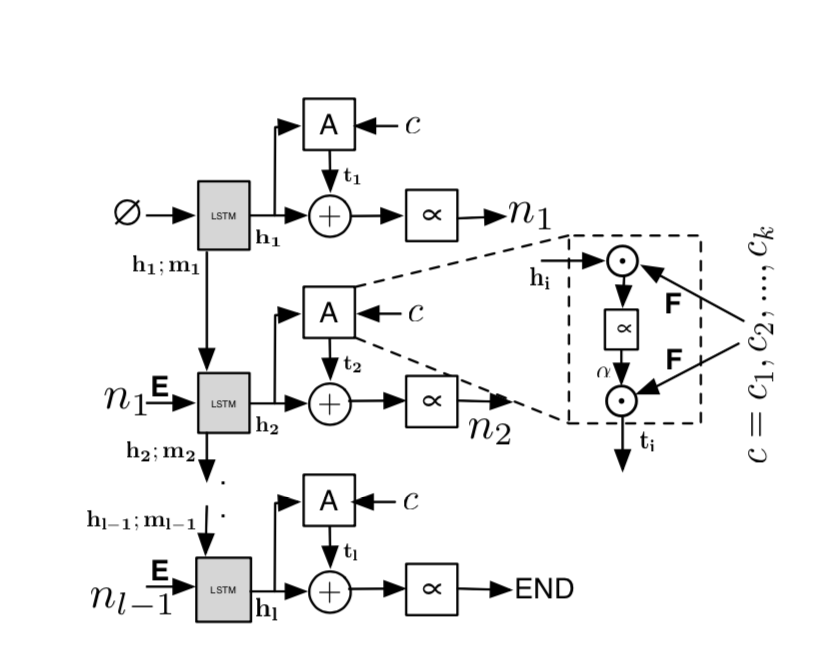
\includegraphics[width=0.5\linewidth]{ModelPics/Iyer_etal.png}
    \caption{Iyer et als Code NN, taken from \cite{iyer_summarizing_2016}}
    \label{fig:Iyer}
\end{figure}


